\chapter{Cadre général du projet}

J’ai rejoint Sopra HR Software Tunisie avec pour mission de digitaliser un processus de recrutement resté, jusque-là, largement manuel. Ce chapitre revient sur le point de départ de ce travail : l’entreprise qui m’a accueilli, les lacunes que j’ai concrètement constatées dans l’existant, la problématique qui en découle, et la manière dont j’ai organisé mon travail sur toute la période de développement de ce Projet de Fin d’Études.

\section{Introduction}
\label{sec_1_1}
Je situe d’abord le cadre organisationnel du projet JOB4YOU, avant de détailler la démarche qui m’a mené à la solution finalement retenue.

\section{Présentation de l’organisme d’accueil}
\label{sec_1_2}
\subsection{Le groupe Sopra Steria}
\label{sec_1_2_1}
Sopra Steria est un groupe européen de conseil, de services numériques et d’édition de logiciels, reconnu pour son expertise sectorielle et son approche de bout en bout sur les projets de transformation numérique. Né du rapprochement entre Sopra Group et Steria en 2014 \cite{ref01}, il rassemble plusieurs dizaines de milliers de collaborateurs répartis dans de nombreux pays, et intervient auprès de grands comptes et d’administrations publiques dans des secteurs variés — finance, télécommunications, énergie, secteur public, ou encore ressources humaines.

\subsection{Sopra HR Software}
\label{sec_1_2_2}
Sopra HR Software est la filiale du groupe spécialisée dans l’édition de solutions logicielles pour la gestion des ressources humaines : paie, gestion administrative du personnel, gestion des talents et gestion du recrutement. En Tunisie, l’entité constitue un centre de développement et de compétences qui contribue à la conception, au développement et à la maintenance des solutions du groupe, tout en gérant en interne ses propres processus, dont le recrutement.

C’est précisément pour répondre à ce besoin interne de digitalisation que le projet JOB4YOU m’a été proposé.

\section{Étude de l’existant}
\label{sec_1_3}
Avant la mise en place du projet, le processus de recrutement au sein de Sopra HR Software reposait sur une combinaison d’outils disparates et de tâches manuelles :

\begin{itemize}
\item La publication des offres d’emploi et leur diffusion s’effectuaient de manière peu centralisée, sans visibilité unifiée sur l’ensemble des postes ouverts.
\item La réception des candidatures et des CV se faisait principalement par messagerie électronique, rendant leur classement, leur archivage et leur consultation fastidieux.
\item Le suivi de l’avancement d’une candidature (CV reçu, examiné, entretien planifié, décision) n’était pas formalisé dans un outil unique, ce qui entraînait une perte d’information entre les différents intervenants (RH, managers).
\item La planification des entretiens et la collecte des feedbacks des managers se faisaient de manière informelle, sans traçabilité ni historique structuré.
\item Aucune notification automatique n’informait les candidats de l’état d’avancement de leur candidature, ce qui pouvait nuire à leur expérience et à l’image de l’entreprise.
\item L’évaluation initiale des candidatures reposait entièrement sur l’analyse manuelle des CV par les équipes RH, un processus chronophage à mesure que le volume de candidatures augmente.
\end{itemize}

Il existe sur le marché des logiciels de suivi des candidatures (ATS, Applicant Tracking System) tels que Workday Recruiting, SAP SuccessFactors Recruiting, Greenhouse ou les modules de recrutement des grands SIRH. Ces outils couvrent la diffusion d’offres, le suivi des candidatures et la planification d’entretiens, mais ils sont pensés pour de grands groupes, coûteux à licencier et à paramétrer, et rarement adaptés au périmètre et aux contraintes d’une entité locale. JOB4YOU se positionne comme une alternative interne, sur mesure et maîtrisée : il reprend les fonctions essentielles d’un ATS (pipeline de candidatures, entretiens, feedbacks, décision finale) tout en y ajoutant un scoring IA des CV paramétrable par famille de métier, un matching inverse « Job idéal » et un assistant conversationnel candidat, le tout intégré aux processus et aux rôles propres à Sopra HR Software Tunisie.

\section{Critique de l’existant et problématique}
\label{sec_1_4}
Cette analyse de l’existant fait ressortir plusieurs limites majeures. Sans outil centralisé, l’information se disperse entre plusieurs canaux — e-mails, fichiers, échanges oraux — ce qui complique la collaboration entre responsables RH et managers impliqués dans la décision de recrutement. Le manque de traçabilité des décisions et des statuts rend le suivi de chaque candidature difficile et allonge les délais de traitement. L’absence d’automatisation, enfin, que ce soit dans la présélection des candidats ou dans la communication avec eux, freine l’efficacité et la scalabilité du processus, surtout à mesure que le volume de candidatures grandit.

De ces constats découle la problématique suivante : comment centraliser, sécuriser et automatiser l’ensemble du processus de recrutement — de la publication d’une offre jusqu’à la décision finale — tout en offrant une visibilité en temps réel à tous les acteurs concernés (administrateurs, RH, managers et candidats) ?

\section{Objectifs du projet}
\label{sec_1_5}
Pour répondre à cette problématique, les objectifs suivants ont été fixés pour ce Projet de Fin d’Études :

\begin{itemize}
\item Concevoir et développer une plateforme web unique regroupant l’ensemble des étapes du processus de recrutement.
\item Mettre en place une gestion des rôles et des accès (Administrateur, RH, Manager, Candidat) garantissant que chaque acteur dispose des fonctionnalités et de la visibilité correspondant à son périmètre.
\item Sécuriser les échanges et les accès à la plateforme via un mécanisme d’authentification robuste (JSON Web Token).
\item Automatiser la pré-analyse des candidatures grâce à un système de scoring assisté par intelligence artificielle, afin d’accélérer le tri initial des CV tout en laissant la décision finale aux équipes RH et managers.
\item Intégrer un système de notifications automatiques par e-mail informant les candidats et les parties prenantes internes à chaque étape clé du processus.
\item Fournir aux équipes RH des outils de pilotage (tableau Kanban, tableau de bord, indicateurs) permettant un suivi visuel et en temps réel de l’avancement des recrutements.
\end{itemize}

\section{Présentation de la solution proposée : JOB4YOU}
\label{sec_1_6}
La solution proposée, baptisée JOB4YOU, est une plateforme web de gestion du processus de recrutement structurée autour de cinq profils d’utilisateurs :

\begin{itemize}
\item Le Visiteur, utilisateur non authentifié, qui consulte et recherche les offres d’emploi publiées et obtient des suggestions « Job idéal » en déposant son CV.
\item Le Candidat, utilisateur authentifié, qui soumet une candidature accompagnée de son CV, suit l’état d’avancement de son dossier et peut échanger avec l’assistant conversationnel.
\item Le Responsable RH, qui publie et gère les offres d’emploi, examine les candidatures reçues, valide les dossiers, planifie les entretiens et contresigne la décision finale — embauche (avec date de présentation des documents) ou refus motivé —, seule étape qui déclenche l’e-mail de réponse au candidat.
\item Le Manager, qui intervient à partir de l’entrée du dossier en évaluation technique (statut TECHNICAL\_TEST), mène ou participe aux entretiens, fournit un feedback structuré et émet un avis — favorable (ACCEPTED) ou refus proposé (MANAGER\_REJECTED) — sur les dossiers de son périmètre ; cet avis est tracé dans le journal d’audit et transmis au RH, qui le contresigne.
\item L’Administrateur, qui supervise la plateforme dans son ensemble, gère les comptes utilisateurs, les rôles et les paramètres globaux du système, notamment ceux liés au scoring par intelligence artificielle.
\end{itemize}

Techniquement, la plateforme s’appuie sur une architecture découplée : un back-end Spring Boot expose des API REST sécurisées, un front-end Angular porte l’interface utilisateur, PostgreSQL sert de base de données relationnelle, et des agents d’automatisation n8n prennent en charge l’analyse des CV par intelligence artificielle (via l’API de Cohere) ainsi que l’envoi des notifications aux différents acteurs. Le chapitre consacré à la conception détaille cette architecture.

\section{Méthodologie de travail adoptée}
\label{sec_1_7}
\subsection{Cadres méthodologiques envisagés}
\label{sec_1_7_1}
Trois cadres sont couramment rencontrés dans les projets de développement. Le modèle en cascade ordonne strictement les phases — analyse, conception, implémentation, tests, déploiement —, chaque phase ne commençant qu’après validation de la précédente ; il convient lorsque le périmètre est stabilisé d’avance, mais encaisse mal l’évolution des besoins, une erreur de conception n’étant généralement découverte qu’en fin de cycle. Le cycle en V conserve cette séquentialité en y adjoignant, pour chaque niveau de conception, un niveau de vérification correspondant, ce qui renforce la traçabilité des tests au prix d’une exigence identique : figer les spécifications très tôt. Scrum \cite{ref02} découpe au contraire le projet en sprints courts à l’issue desquels un incrément potentiellement livrable est présenté ; les exigences y sont portées par un backlog produit priorisé en continu, et le cadre s’appuie sur des rôles — Product Owner, Scrum Master, équipe de développement — et des cérémonies — planification de sprint, mêlée quotidienne, revue de sprint, rétrospective — formalisés.

\subsection{Cadre retenu et transposition au travail individuel}
\label{sec_1_7_2}
J’ai retenu Scrum comme cadre de référence, pour une raison tenant au contenu du projet : son périmètre n’était pas stabilisable d’avance. Le barème de scoring par intelligence artificielle — seuil de décision, zone d’incertitude laissée autour de lui, place de l’arbitrage humain — et la part confiée aux agents d’automatisation n8n ont été arbitrés au fil de l’eau, entre le printemps et l’automne 2026. Un cycle en V aurait exigé de figer dès mars 2026 des règles de décision qui ne sont devenues opérationnelles que plusieurs mois plus tard ; la cascade aurait, elle, repoussé la confrontation au réel de la plateforme jusqu’à la fin du stage. Le cadre agile impose en outre un point de validation à chaque fin de cycle, ce qui correspondait exactement au rythme des suivis assurés par mon encadrant entreprise.

Restait à transposer dans un projet mené par une seule personne un cadre conçu pour des équipes de trois à neuf développeurs. Plutôt que de déclarer une adhésion formelle à Scrum ou de l’écarter, j’en ai repris les éléments qui ont un équivalent réel dans ce contexte et assumé l’absence des autres ; le tableau~\ref{tab_1_1} explicite cette transposition, élément par élément.

% tableau 1.1
\setcounter{table}{0}
\begin{table}[!ht]
\centering
\caption{Transposition du cadre Scrum au projet}
\label{tab_1_1}
\renewcommand{\arraystretch}{1.25}\footnotesize
\setlength{\tabcolsep}{4pt}%
\begin{tabular}{|P{0.235\textwidth}|P{0.695\textwidth}|}
\hline
\textbf{Élément du cadre Scrum} & \textbf{Transposition retenue dans le projet} \\
\hline
Product Owner & Mon encadrant entreprise : il exprime le besoin, arbitre les priorités à chaque point d’avancement et accepte l’incrément lors de la démonstration \\
\hline
Scrum Master & Sans équivalent formel : à une seule personne, la facilitation — cadrage du sprint, arbitrage des dépendances techniques — est confondue avec le rôle de développeur \\
\hline
Équipe de développement & Une seule personne (l’auteur de ce rapport) : conception, développement, tests et déploiement sur l’environnement de développement \\
\hline
Sprint & Cycle d’environ quatre semaines d’avril à septembre 2026, puis deux sprints resserrés à deux semaines en octobre (tableau~\ref{tab_1_3}) \\
\hline
Backlog produit & Liste ordonnée des user stories issues de l’analyse de l’existant et des retours de démonstration (tableau~\ref{tab_1_4}) \\
\hline
Planification de sprint & En début de cycle, sélection des user stories à traiter, chacune étant assortie d’un critère de sortie vérifiable en démonstration \\
\hline
Revue de sprint & Démonstration de l’incrément fonctionnel à l’encadrant entreprise en fin de cycle ; ses retours déterminent le contenu du cycle suivant \\
\hline
Rétrospective & Point d’ajustement à l’issue de chaque démonstration : ce qui bloque, ce qui est reporté, ce qui doit être repris \\
\hline
Mêlée quotidienne & Remplacée, en travail individuel, par un suivi d’avancement hebdomadaire avec l’encadrant entreprise \\
\hline
Incrément et définition de « fini » & Incrément compilé, testé (tests unitaires et fonctionnels), déployé sur l’environnement de développement et démontrable sans échec visible \\
\hline
Vélocité et diagramme de burndown & Non produits : aucune mesure de vélocité n’a été tenue pendant le stage ; le suivi s’est fait par jalons de démonstration \\
\hline
\end{tabular}
\end{table}
Cette transposition a une limite, qu’il vaut poser ici plutôt que de la laisser deviner : le backlog et la vélocité n’ont pas été tenus en temps réel. Le tableau~\ref{tab_1_4} présente un backlog reconstitué à partir du code livré et des comptes rendus de démonstration, et la décomposition en sprints du tableau~\ref{tab_1_3} suit les repères mensuels du stage, non un relevé de charge quotidien. Git/GitHub a servi d’outil de versionnage et de retour en arrière ; son historique, plus dense sur la seconde moitié de la période, n’atteste pas le rythme de développement et n’est donc pas invoqué comme preuve méthodologique.

\section{Planification du projet}
\label{sec_1_8}
\subsection{Macro-planification des phases}
\label{sec_1_8_1}
La période de réalisation s’étend de février à octobre 2026. Elle a d’abord été planifiée par grandes phases, alignées sur les jalons de suivi académiques et industriels du stage, afin de concilier la souplesse des sprints avec des repères communicables à l’école et à l’entreprise. Ces phases sont résumées dans le tableau~\ref{tab_1_2}.

% tableau 1.2
\setcounter{table}{1}
\begin{table}[!ht]
\centering
\caption{Macro-planification des phases du projet}
\label{tab_1_2}
\renewcommand{\arraystretch}{1.25}\footnotesize
\setlength{\tabcolsep}{4pt}%
\begin{tabular}{|P{0.197\textwidth}|P{0.103\textwidth}|P{0.646\textwidth}|}
\hline
\textbf{Phase} & \textbf{Repère mensuel} & \textbf{Activités principales} \\
\hline
Prise en main et cadrage & Février 2026 & Intégration au sein de l’équipe, étude de l’existant, analyse du besoin, rédaction du cahier des charges \\
\hline
Analyse et conception & Mars 2026 & Spécification des besoins, modélisation UML \cite{ref03} (cas d’utilisation, séquence, classes), conception de la base de données \\
\hline
Développement — socle applicatif (release 1) & Avril – Mai 2026 & Mise en place de l’architecture back-end/front-end, authentification JWT, gestion des rôles, gestion des offres et des candidatures \\
\hline
Développement — fonctionnalités avancées (release 2) & Juin – Août 2026 & Scoring IA des CV, agents n8n et notifications e-mail, entretiens et feedbacks, tableau Kanban, calendrier, suggestions « Job idéal » et assistant conversationnel \\
\hline
Fiabilisation et durcissement (release 3) & Septembre 2026 & Tests fonctionnels de bout en bout, corrections de bugs, reprise des erreurs des agents d’automatisation, améliorations UX et sécurité \\
\hline
Évaluation, recette et soutenance (release 4) & Octobre 2026 & Évaluation du scoring sur Gold Set et calibrage du seuil, jeu de démonstration, relecture du rapport avec l’encadrant, préparation de la soutenance \\
\hline
\end{tabular}
\end{table}
La figure~\ref{fig_1_1} reprend ces phases sur le calendrier mensuel de février à octobre 2026 ; ses deux bandes inférieures superposent les quatre releases et les huit sprints qui en découlent.

% figure 1.1
\setcounter{figure}{0}
\begin{landscape}
\pagestyle{lscape}
\begin{figure}[p]
\centering
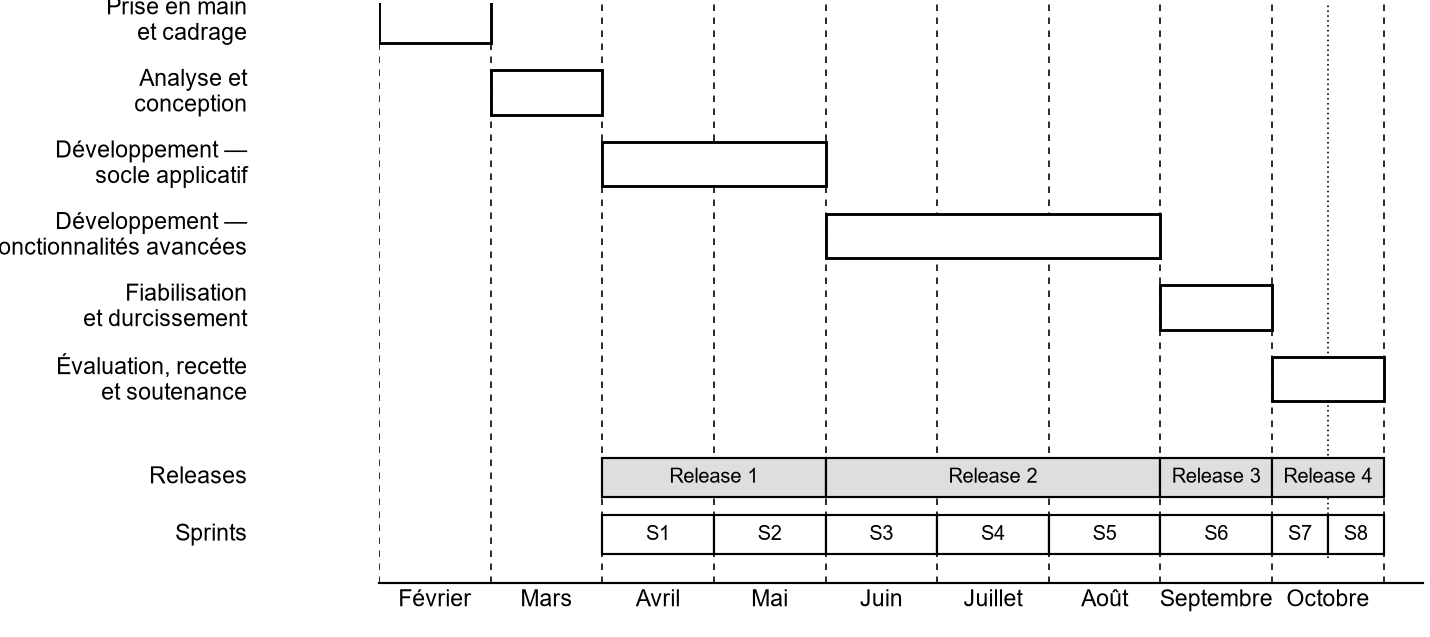
\includegraphics[width=0.98\linewidth, height=0.90\textheight, keepaspectratio]{fig1_1}
\caption{Diagramme de Gantt — Planification mensuelle des phases du projet}
\label{fig_1_1}
\end{figure}
\clearpage
\end{landscape}

\subsection{Découpage en sprints et en releases}
\label{sec_1_8_2}
La période de développement — d’avril à octobre 2026 — a été découpée en huit sprints : six sprints d’environ quatre semaines d’avril à septembre, puis deux sprints resserrés à deux semaines en octobre, à l’approche de la soutenance. Les deux premiers mois du stage sont restés hors sprint, consacrés à la prise en main de l’environnement, à l’analyse du besoin et à la conception UML : aucun incrément démontrable n’y était attendu. Chaque sprint regroupait les user stories prioritaires restantes et se terminait par une revue avec l’encadrant entreprise ; le détail en est donné au tableau~\ref{tab_1_3}.

Quatre releases agrègent ces sprints, chacune correspondant à un incrément complet du point de vue de l’utilisateur : la release 1 rend le cycle de candidature opérationnel, la release 2 dote la plateforme de son aide à la décision, la release 3 fiabilise l’ensemble et la release 4 l’évalue avant sa présentation finale.

% tableau 1.3
\setcounter{table}{2}
\begin{table}[!ht]
\centering
\caption{Découpage en sprints et en releases (avril – octobre 2026)}
\label{tab_1_3}
\renewcommand{\arraystretch}{1.25}\footnotesize
\setlength{\tabcolsep}{4pt}%
\begin{tabular}{|P{0.050\textwidth}|P{0.125\textwidth}|P{0.400\textwidth}|P{0.325\textwidth}|}
\hline
\textbf{Sprint} & \textbf{Période} & \textbf{Objectif du sprint} & \textbf{Critère validé en revue} \\
\hline
S1 & Avril 2026 & Mettre en place le socle technique : architecture back-end Spring Boot et front-end Angular, schéma PostgreSQL, authentification JWT et gestion des rôles & Les applications démarrent ensemble ; un compte par rôle se connecte et n’accède qu’à son périmètre \\
\hline
S2 & Mai 2026 & Cycle de base candidat–offre : publication et gestion des offres, dépôt de candidature avec CV, suivi de l’état du dossier & Une candidature est créée, déposée et suivie de bout en bout par le candidat et par le RH — clôture la release 1 \\
\hline
S3 & Juin 2026 & Présélection assistée : extraction du texte du CV, scoring sur 100 via l’API de Cohere, agents n8n et notifications e-mail & Un CV déposé est noté, la règle de décision appliquée et tracée dans le journal d’audit ; les notifications partent \\
\hline
S4 & Juillet 2026 & Pipeline RH/manager : planification des entretiens, feedbacks structurés, avis du manager contre-signé par le RH, tableau Kanban & Un dossier traverse présélection, entretiens et décision finale avec ses notifications \\
\hline
S5 & Août 2026 & Fonctions d’accompagnement : suggestions « Job idéal » (matching inverse), assistant conversationnel côté candidat, calendrier d’entretiens avec rappels & Les trois fonctions sont utilisables par un candidat et par un manager — clôture la release 2 \\
\hline
S6 & Septembre 2026 & Fiabilisation : tests fonctionnels de bout en bout, corrections de bugs, reprise des erreurs des agents d’automatisation, durcissement de la sécurité et de l’UX & Le scénario complet de démonstration s’exécute sans échec visible — clôture la release 3 \\
\hline
S7 & Octobre (1re quinzaine) & Évaluation du scoring : constitution du Gold Set de vingt CV, mesure à trois seuils, zone d’incertitude et réévaluation manuelle par le RH & Matrice de confusion et métriques produites, commentées puis intégrées au chapitre~4 \\
\hline
S8 & Octobre (2e quinzaine) & Recette finale et préparation de la soutenance : jeu de démonstration, enregistrement vidéo, relecture du rapport avec l’encadrant & Rapport et support de soutenance validés par l’encadrant entreprise — clôture la release 4 \\
\hline
\end{tabular}
\end{table}

\subsection{Backlog reconstitué des user stories}
\label{sec_1_8_3}
Le tableau~\ref{tab_1_4} rattache les user stories des principales fonctionnalités livrées à leur acteur bénéficiaire et à la release qui les a vues aboutir.

% tableau 1.4
\setcounter{table}{3}
\begin{table}[!ht]
\centering
\caption{Backlog reconstitué des user stories par release}
\label{tab_1_4}
\renewcommand{\arraystretch}{1.25}\footnotesize
\setlength{\tabcolsep}{4pt}%
\begin{tabular}{|P{0.430\textwidth}|P{0.140\textwidth}|P{0.375\textwidth}|}
\hline
\textbf{User story} & \textbf{Acteur bénéficiaire} & \textbf{Release (période 2026)} \\
\hline
Créer un compte et postuler à une offre (dépôt du CV) & Candidat & Release 1 — avril – mai \\
\hline
Suivre l’avancement de sa candidature à chaque étape & Candidat & Release 1 — avril – mai \\
\hline
Publier et gérer les offres d’emploi du périmètre RH & Responsable RH & Release 1 — avril – mai \\
\hline
Faire présélectionner les CV par un score IA paramétrable & Responsable RH & Release 2 — juin – août \\
\hline
Planifier les entretiens, émettre un avis et le contresigner & RH et Manager & Release 2 — juin – août \\
\hline
Consulter le tableau Kanban et le journal d’audit & Responsable RH & Release 2 — juin – août \\
\hline
Disposer d’un calendrier d’entretiens avec rappels & Manager & Release 2 — juin – août \\
\hline
Bénéficier des suggestions « Job idéal » et du chatbot & Candidat & Release 2 — juin – août \\
\hline
Exécuter un cycle complet sans régression visible & RH, Manager et Candidat & Release 3 — septembre \\
\hline
Évaluer, corriger et expliquer le scoring IA & Responsable RH & Release 4 — octobre \\
\hline
\end{tabular}
\end{table}

Backlog reconstitué a posteriori à partir du code livré et des comptes rendus de démonstration, non tenu en temps réel durant le stage ; les repères mensuels sont ceux de la macro-planification du tableau~\ref{tab_1_2} et n’ont donné lieu à aucune mesure de vélocité.
\section{Conclusion}
\label{sec_1_9}
Les limites du processus existant chez Sopra HR Software sont maintenant posées, tout comme la méthodologie suivie pendant le stage. Reste à entrer dans le vif du sujet : quels besoins précis JOB4YOU devait-il couvrir ? C’est l’objet du chapitre suivant.
